\documentclass[tikz,border=8pt]{standalone}
\usepackage{tikz}
\usepackage{tkz-euclide}
\usepackage{amsmath, amssymb}

\usetikzlibrary{angles, quotes}

\begin{document}

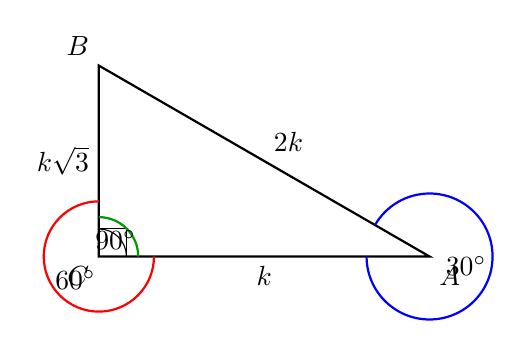
\begin{tikzpicture}[scale=1.4]

  % ---- Vértices del triángulo rectángulo 30°-60°-90° ----
  \coordinate (C) at (0,0);   % ángulo recto
  \coordinate (A) at (3,0);   % ángulo de 30° (opuesto al cateto menor)
  \coordinate (B) at (0,1.732); % ángulo de 60° (√3 ≈ 1.732)

  % ---- Lados del triángulo ----
  \draw[thick] (A) -- (B) -- (C) -- cycle;

  % ---- Ángulo recto en C ----
  \draw (0.25,0) arc (0:90:0.25);
  \draw (0,0.25) -- (0.25,0.25) -- (0.25,0);

  % ---- Marcas de ángulos ----
  \pic["$30^\circ$", draw=blue, thick, angle radius=0.8cm] {angle=C--A--B};
  \pic["$60^\circ$", draw=red, thick, angle radius=0.7cm] {angle=B--C--A};
  \pic["$90^\circ$", draw=green!60!black, thick, angle radius=0.5cm] {angle=A--C--B};

  % ---- Etiquetas de lados ----
  \node[below] at (1.5,0) {$k$};
  \node[left] at (0,0.866) {$k\sqrt{3}$};
  \node[above right] at (1.5,0.866) {$2k$};

  % ---- Etiquetas de vértices ----
  \node[below left] at (C) {$C$};
  \node[below right] at (A) {$A$};
  \node[above left] at (B) {$B$};

  % ---- Altura desde B hacia AC (opcional, trazo auxiliar) ----
  % \draw[dashed] (B) -- (0,0);

\end{tikzpicture}

\end{document}
